\chapter{Polarization Rotator} \label{cha:polrot} \index{Polarization!rotator|(}

\section{Introduction}

Building a polarization rotator\index{Polarization!rotator} is
probably the most challenging step in implementing a polarization
diversity\index{Polarization!diversity} scheme. While several concepts
for polarization splitters are available (\cite{kiyat_compact},
\cite{taillaert_compact}, \cite{wu_planar}), available polarization
rotators can be subdivided in two big families, based on two opposite
physical principles.
\begin{description}
\item[Adiabaticity]\index{Adiabaticity}, or
  mode-evolution\index{Mode!evolution} principle: an input
  birefringent waveguide\index{Waveguide!birefringent}, in which the
  effective index\index{Effective!index} of one polarization is
  greater than the other one, is adiabatically transformed into
  another birefringent waveguide, for which the effective indices
  associated to orthogonal polarizations are swapped. If the
  transition is adiabatic, power into one mode do not couple to other
  modes: if the higher index mode is excited at the input, power stays
  on the higher index mode, that, at the output, has the orthogonal
  polarization. There are many ways to achieve this transition, all of
  them sharing the characteristic that the transition from the input
  waveguide to the output one must be done asymmetrically: this is
  needed to prevent symmetry from forcing one polarization to stay in
  the same polarized mode. A very simple example of polarization
  rotator in the microwave regime is a rectangular waveguide twisted
  of $90\degrees$ around its axis: if the twist is slow enough, the
  input TE mode (for example, with higher effective index) is
  ``bended'' into the output TM mode (again with the higher effective
  index) without reflections, and viceversa. In planar integrated
  optics, the twisting of a dielectric waveguide is not feasible, but
  ``effective twisting'' structures can be realized, based on the same
  idea: see \cite{watts_integrated} for a successful adiabatic
  design. The advantages of adiabaticity are a fabrication tolerant
  and inherently broadband design. The main disadvantage is a very
  long device, up to hundreds of microns for optical frequencies,
  necessary to achieve adiabaticity.
\item[Mode coupling]\index{Mode!coupling}: an input mode, with a given
  polarization, is used to excite two or more modes of a device which
  support modes with hybrid polarization\index{Polarization!hybrid}
  and different propagation constants. Power flows from one hybridly
  polarized mode to the others and, after a fixed propagation length
  (the beat length\index{Beat length}), polarization is rotated as
  desired. To have complete rotation, i.e. no crosstalk, the hybrid
  modes must be phase matched\index{Phase matching}, the hybrid modes
  linearly polarized at $\pm 45\degrees$ and the total device length
  finely tuned. This results in a fabrication intolerant and
  wavelength sensitive device. Many authors have presented different
  designs: see \cite{huang_realization}, \cite{tzolov_passive}, \cite{lui_polarization},
  \cite{kotlyar_compact}, \cite{correia_genetic},
  \cite{elrefaei_slanted}, for example. The main advantage over
  adiabatic devices is that such devices can be very short: in
  \cite{kotlyar_compact} a $1.6 \mu m$ long polarization rotator is
  presented, which is also reasonably broadband. In fact, making a
  very short device has the double advantage of saving space on the
  optical chip and making the device broadband: if mode coupling only
  happens on a short distance, then the ``filtering'' property of the
  device is relaxed and so its frequency selectivity.
\end{description}

The device studied in this chapter is based on mode coupling: the
advances of technological processes have convinced the Author of the
possibility to achieve the same performances of adiabatic devices --
in theory, $100\%$ conversion -- in a much shorter device. Moreover, a
short polarization rotator could be used for other integrated devices,
such as Solc filters \cite{solc_birefringent}, and the same principle
could be used to rotate the polarization of an arbitrary angle, not
only $90\degrees$: definitely, a more flexible device than the
adiabatic one.

The key difficulty in realizing it is to create a waveguide that
supports two orthogonally polarized modes, $A$ and $B$ in
\figref{fig:polrot_modes}, at $\pm 45\degrees$, with different
effective indices\index{Effective!index} $n_{eff}^{\pm 45}$. The resulting waveguide behaves
as a half-wave plate: the input mode, polarized at $0\degrees$ ($A+B$),
or $90\degrees$ ($A - B$), excites both of them with the same amount
of power and, after a length $L_\pi =
\frac{\lambda}{2\Abs{n_{eff}^{+45} - n_{eff}^{-45}}}$, corresponding
to a $\pi$ phase shift of the two modes $A$ and $B$, the polarization
has been rotated by $90\degrees$, as desired.

\begin{figure}[htbp]
  \begin{center}
    \resizebox{5cm}{!}{\input{pics/polrot_modes.pdf_t}}
  \end{center}
  \caption{$\pm45\degrees$ linearly polarized modes. An input
    vertically polarized mode $A+B$ excites both $A$ and $B$: after
    $L_\pi$, $A$ and $B$ are phase shifted by $\pi$ and the resulting
    field $A - B$ is horizontally polarized.}
  \label{fig:polrot_modes}
\end{figure}

This condition has been previously realized by etching a rib waveguide
with one straight and one slanted sidewall \cite{elrefaei_slanted}
\cite{elrefaei_optimized}. The resulting device is hundreds of microns
long, though: not better, in length, than an adiabatic one. The effect
of the slanted wall is not strong enough to induce a large
birefringence $\Delta n = n_{eff}^{+45} - n_{eff}^{-45}$, necessary
for a small $L_\pi$.

Inspired from \cite{cai_ultra}, the effect of a slanting edge
in the waveguide can be enhanced using a one-dimensional photonic
crystal. The idea consists in using fabrication techniques typically
used in photonic crystal devices to etch deep air slots, slated at a
certain angle, into a conventional ridge waveguide.

The complete device, fabricated by the University of St. Andrews, is
presented in \cite{kotlyar_compact} and
\cite{bolla_funfox_losanna}. After a short description of the wafer,
the design and the optimization process will be described and,
finally, simulated and measured results will be compared.

\section{Description of the Wafer}

The InGaAsP heterostructure (grown by Alcatel) used in the experiments
consists of a $0.3 \mu m$-thick InP top cladding layer and a $0.522
\mu m$ InGaAsP (Q 1.22) core layer, followed by InP lower cladding
\figref{fig:polrot_experimental_device}.

\begin{figure}[htbp]
  \begin{center}
    \subfigure[Cross section.]{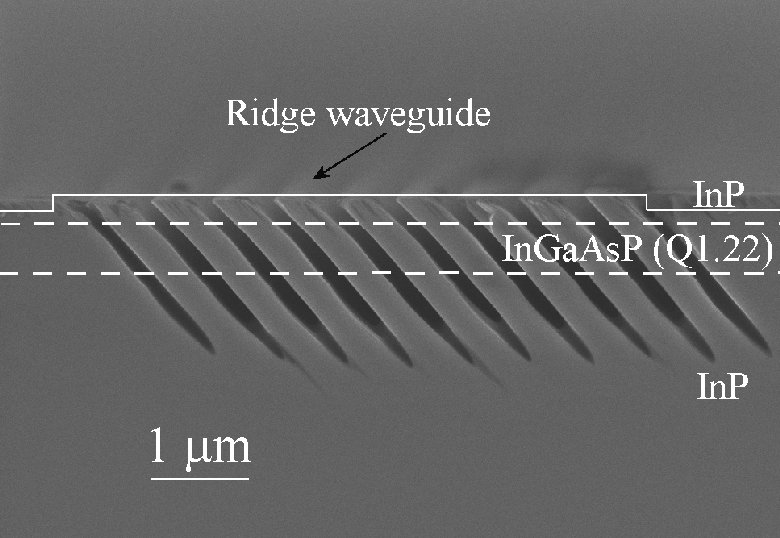
\includegraphics[width=8cm]{pics/polrot_experimental_section}}
    \subfigure[Top view.]{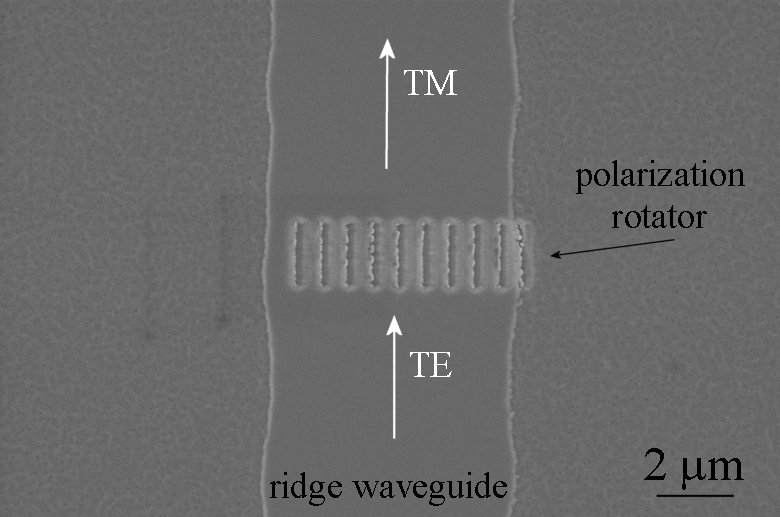
\includegraphics[width=8cm]{pics/polrot_experimental_waveguide}}
  \end{center}
  \caption{Experimental device. Compare it with
  \figref{fig:polrot_wafer}.}
  \label{fig:polrot_experimental_device}
\end{figure}

A set of $230 nm$ slots with a $650 nm$ period was written using
electron-beam lithography (Raith Elphy Plus/Leo 1530) in a $200 nm$
thick layer of poly\-methy\-metha\-cry\-la\-te. The pattern was then transferred
into a hard silica mask using reactive ion etching with fluorine
chemistry (CHF3). The silica mask was created using commercially
available hydrogen silsesquioxane (HSQ) resist that was simply applied
through spin coating. Baking this resist at high temperatures ($\sim
400\degrees C$) partially transforms the film into silica.

The deep etching of the slots was performed using a high voltage low
current chemically assisted ion beam etching (CAIBE) regime at a
temperature of $\sim 200\degrees C$. The sample was mounted on a slanted
holder in order to etch the slots at the desired angle of 45
degrees.

The access input/output ridge waveguides ($5 \mu m$ wide) were defined
using photolithography. The shallow etching ($100 nm$) necessary for
operation in a single mode (as shown in \ref{sec:polrot_design}) was
realized using a second stage of CAIBE etching with the photoresist as
the protective mask. Finally, the sample was cleaved into die of
approximately $1mm$ length.

\section{Design} \label{sec:polrot_design}

Given the wafer described in the previous section, a suitable design
for the polarization rotator must be studied. The optimized design
will be, clearly, strongly wafer-dependent.

The waveguide chosen is a ridge waveguide, as the one shown in
\figref{fig:polrot_wafer}. The ridge width is $5 \mu m$, etched by
$100 nm$ from the air top: these dimensions ensure the monomodality of
the waveguide. In \figref{fig:polrot_ridge} the first TE and first TM
modes of the waveguide without the air slots are shown, computed using
the vectorial mode solver described in
\ref{sec:vectorial_mode_solver}. All the other higher modes are
cutoff.

\begin{figure}[htbp]
  \begin{center}
    \resizebox{!}{5cm}{\input{pics/polrot_wafer_x.pdf_t}}
    \resizebox{!}{5cm}{\input{pics/polrot_wafer_z.pdf_t}}
  \end{center}
  \caption{Wafer's cross section. Compare it with
    \figref{fig:polrot_experimental_device}. All the dimensions are in
    $nm$ if not explicitly stated. The optimization parameters are
    shown: $W$, the air slots width, $A$, the air slots etch angle and
    $P$, the air slots periodicity. The etch depth $D$ is fixed at $1.6
    \mu m$.}
  \label{fig:polrot_wafer}
\end{figure}

\begin{figure}[htbp]
  \begin{center}
    \subfigure[First TE mode.]{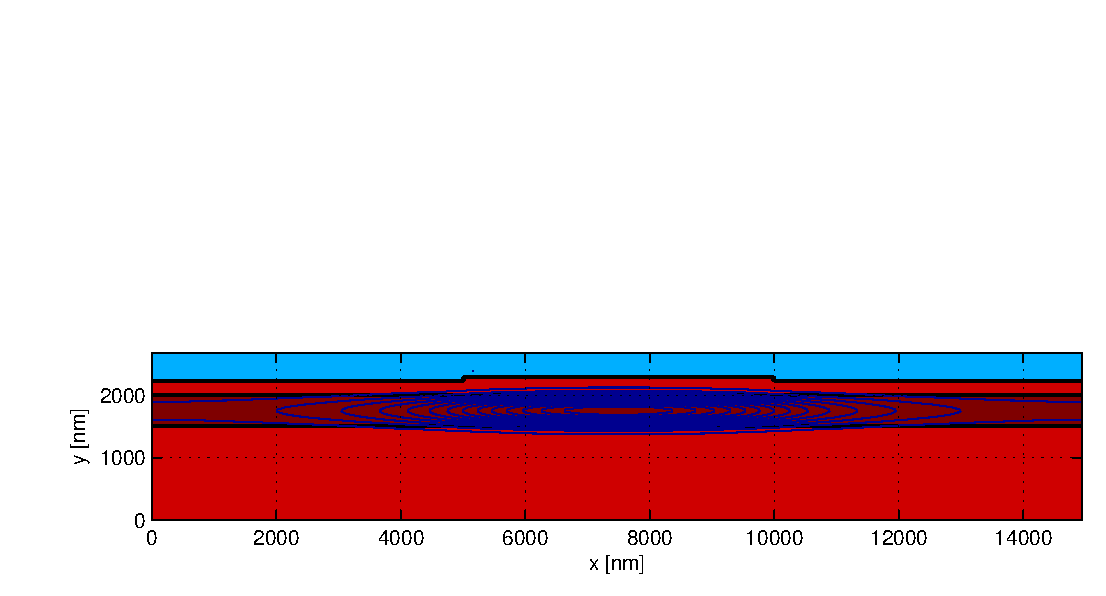
\includegraphics[width=8cm]{pics/polrot_ridge_TE1}}
    \subfigure[First TM mode.]{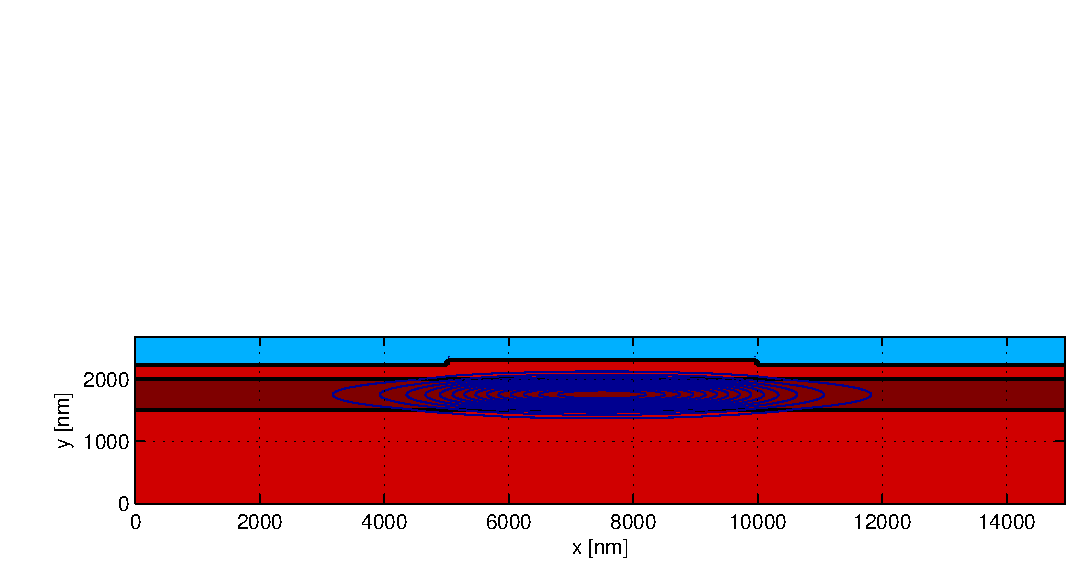
\includegraphics[width=8cm]{pics/polrot_ridge_TM1}}
  \end{center}
  \caption{Contour plot of the longitudinal component of the Poynting
    vector, for the two ridge waveguide modes. The ridge width ($5 \mu
    m$) and depth ($100 nm$) are chosen to have monomodal operation.}
  \label{fig:polrot_ridge}
\end{figure}

In \figref{fig:polrot_wafer}, the optimization parameters are
shown. There are four degrees of freedom in the design of the air
slots:
\begin{enumerate}
\item $W$, the width;
\item $P$, the periodicity;
\item $A$, the etch angle;
\item $D$, the etch depth.
\end{enumerate}

In choosing them, to simplify the design, some design hints are taken
into account:
\begin{itemize}
\item
  the fabrication process can only etch at some given angles: only
  angles between $40\degrees$ and $50\degrees$ are practically
  feasible;
\item
  the periodicity $P$ is always greater than the air slots width $W$,
  by definition, but a $P \gg W$ resembles the case of a common slab
  waveguide, which is well know to support only pure TE and pure TM
  modes: no $\pm45\degrees$ linearly polarized modes are expected in
  this case;
\item
  the larger the air slots, the more mismatched the device will be
  with the input ridge waveguide: all the light that is reflected at
  the interface between the input waveguide and the polarization
  rotator is lost, hence not converted;
\item
  the deeper the air slots, the better, because coupling with the
  substrate is prevented: a feasible working depth of $1.6 \mu m$ has
  been chosen and fixed from now on for the optimization: in
  \figref{fig:polrot_holes} this choice is justified;
\item
  the aspect ratio between the etching depth and the air slots $W/D$
  (or the etching depth and the periodicity $P/D$) is critical for the
  quality of the air slots. Very small aspect ratios are difficult to
  achieve: non-straight walls, wrong widths and depths are the
  consequences;
\item
  the rotation effect increases with the number of the air slots along
  the cross section of the ridge waveguide.
\end{itemize}

Each design parameter has a range of possible values, given by the
fabrication process and the hints above: they are reported in
\tabref{tab:polrot_parameters}. 

\begin{table}[htbp]
  \begin{center}
    \begin{tabular}{ccc}
      \hline
      Parameter & From & To \\
      \hline
      $W$ & $260 nm$ & $280 nm$ \\
      $A$ & $40 \degrees$ & $50 \degrees$ \\
      $P$ & $600 nm$ & $700 nm$ \\      
      \hline
    \end{tabular}
  \end{center}
  \caption{Optimization parameters.}
  \label{tab:polrot_parameters}
\end{table}

The optimization has been done iterating on all the possible
combinations of these parameters, looking for a global maximum of a
certain cost function. In our case, the cost function has been thought
to weight the most important characteristic that the device must have
to work properly. In particular, let $A$ and $B$ be the two modes of
the structure, more similar to the ideal $\pm 45\degrees$ linearly
polarized modes, polarized at angles $\alpha_A$ and $\alpha_B$
respectively. Then:
\begin{enumerate}
\item
  the polarization angle difference between $A$ and $B$ must be equal
  to: $\alpha_A - \alpha_B = \pm 90\degrees$;
\item
  the polarization angle sum between $A$ and $B$ must be equal
  to: $\alpha_A + \alpha_B = 0\degrees$ or $180\degrees$;
\item
  the mode power $P_A$ and $P_B$ (normalized to unity) must be
  concentrated mainly in the core.
\end{enumerate}

The first two points refer to the fact that to have $100\%$ conversion
the modes must be linearly polarized at $\pm 45\degrees$. Their
importance weights $0.4$ each in the cost function. The last point
endsures that the modes are guided by the core and not by the
cladding. This weights $0.2$. The final weight function $C$ is:
\begin{equation} \label{eqn:polrot_weight} \begin{split}
  C & \eqdef 0.4 \left( \frac{\Abs{\alpha_A - \alpha_B}}{90} \right) \\
    & + 0.4 \left( 1 - \frac{\alpha_A + \alpha_B}{180} \right) \\
    & + 0.2 \left( \frac{P_A + P_B}{2} \right)
\end{split} \end{equation}
and it can have values between $0$ and $1$.

\figref{fig:polrot_optimization} shows the cost function $C$ for
different choices of the optimization parameters. As long as $C$ is a
function of three parameters $W$, $A$ and $P$, for ease of
visualization two-dimensional sections are shown: one for constant $A$
and one for $P$.

\begin{figure}[htbp]
  \begin{center}
    \subfigure[$P$-$W$ section at $A = 45\degrees$ constant.]{\label{fig:polrot_optimization:pw}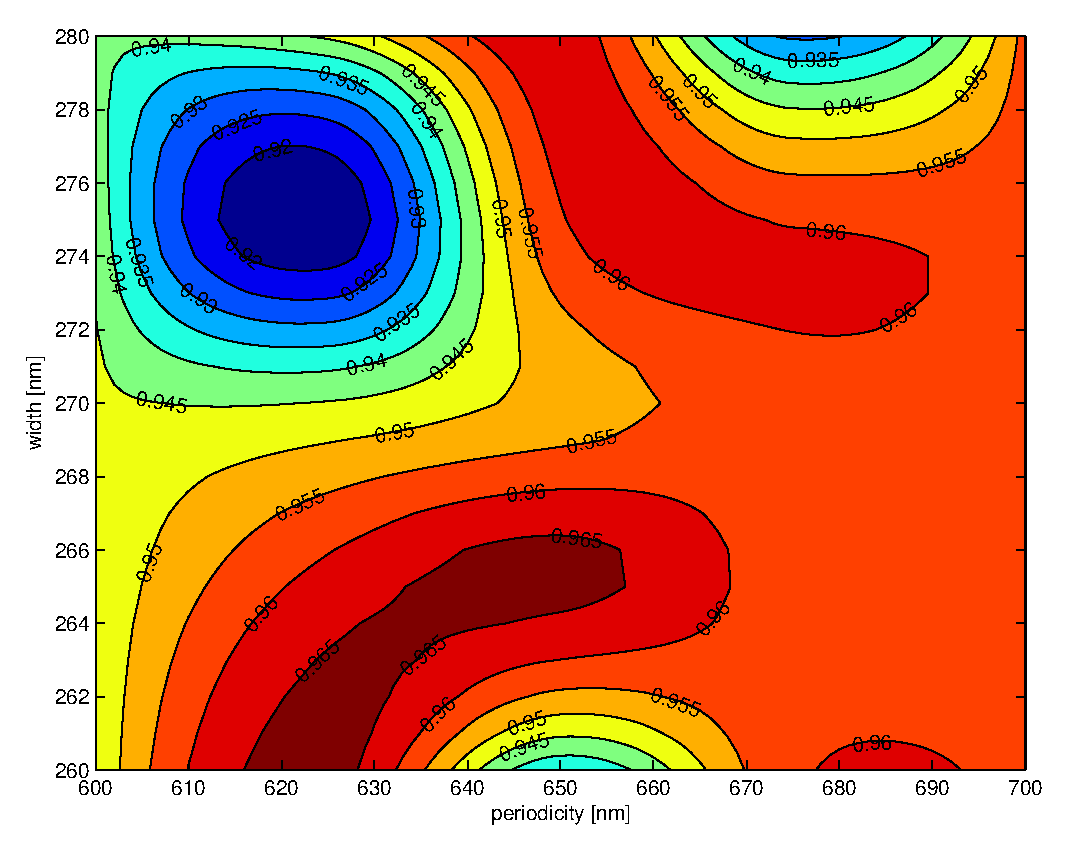
\includegraphics[width=8cm]{pics/polrot_optimization_pw}}
    \subfigure[$A$-$W$ section at $P = 650 nm$ constant.]{\label{fig:polrot_optimization:aw}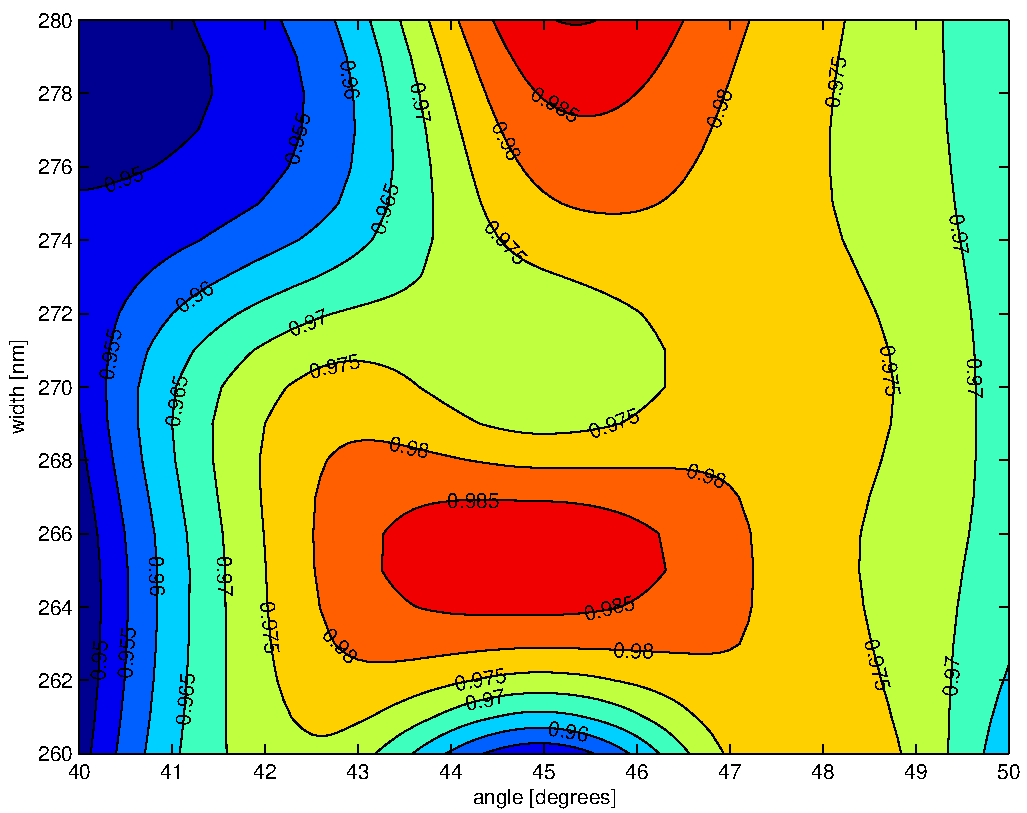
\includegraphics[width=8cm]{pics/polrot_optimization_aw}}
  \end{center}
  \caption{Cost function $C$ as defined in \eqref{eqn:polrot_weight},
    for different choices of the optimization parameters. The chosen
    maximum is for $W = 266 nm$, $A = 45\degrees$ and $P = 650 nm$,
    where $C = 0.97$.}
  \label{fig:polrot_optimization}
\end{figure}

We can note that there is a maximum for $W = 266 nm$\footnote{The
  actual parameter passed to the fabrication process is $W = 270 nm$,
  within the fabrication tolerances.}, $A = 45\degrees$ and $P = 650
nm$: the cost function is $C = 0.97$. The two modes obtained in this
case are shown in \figref{fig:polrot_optimum}. They have the
effective indices\index{Effective!index}:
\begin{align*}
  n_{eff}^{+45} = 3.046 && n_{eff}^{-45} = 2.604
\intertext{and the polarization angles:}
  \alpha^{+45} = 45.1\degrees && \alpha^{-45} = 42.5\degrees.
\end{align*}

The expected beat length\index{Beat length} is $L_\pi = 1.5 \mu m$ at $\lambda = 1300
nm$.

\begin{figure}[htbp]
  \begin{center}
    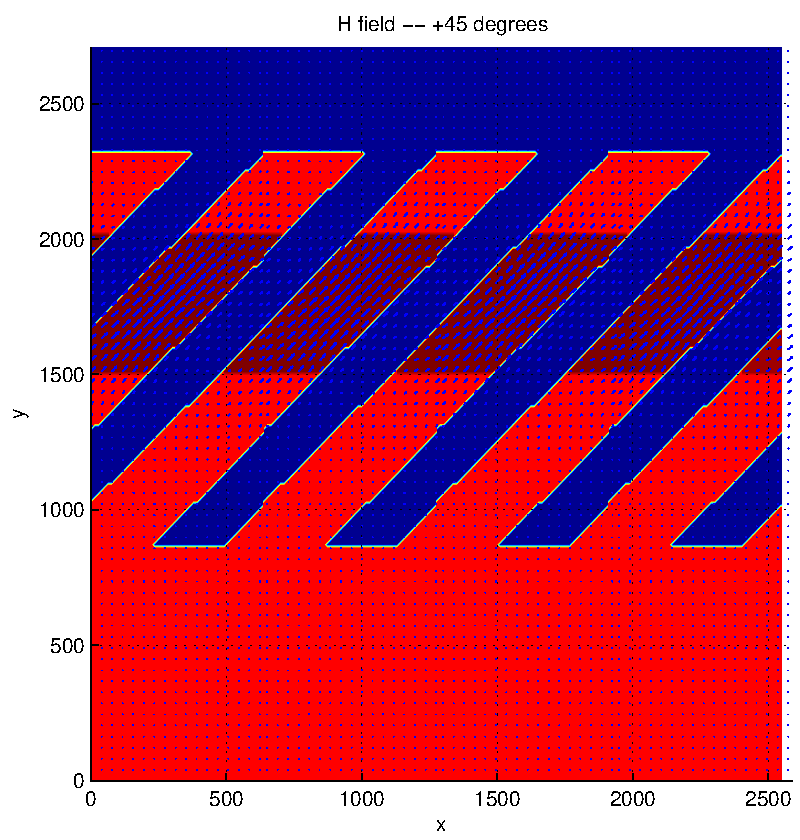
\includegraphics[width=8cm]{pics/polrot_optimum_1}
    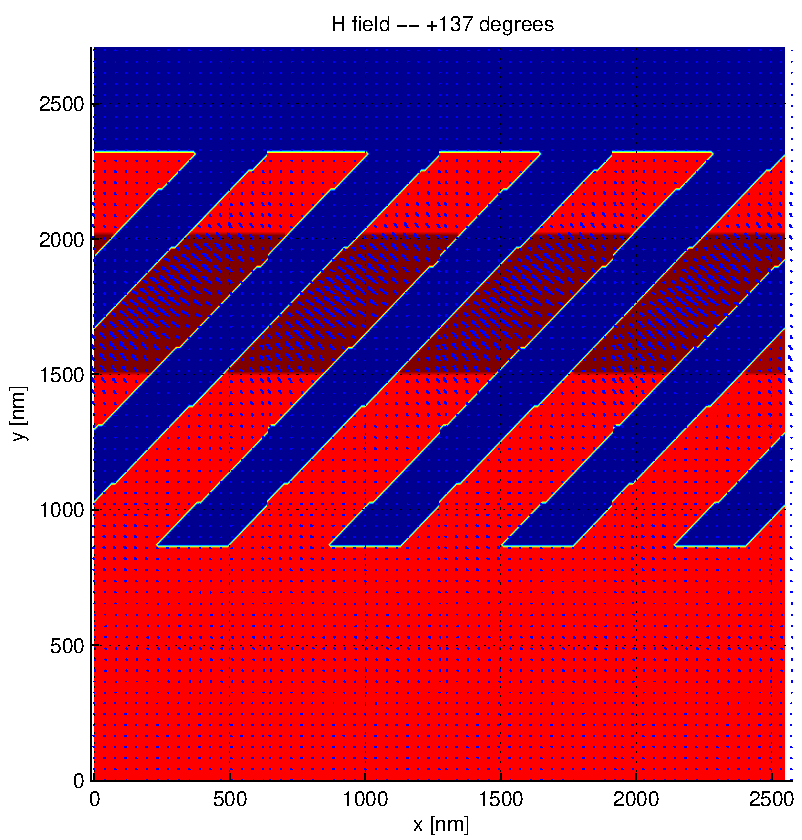
\includegraphics[width=8cm]{pics/polrot_optimum_2}
  \end{center}
  \caption{Magnetic field of the optimum modes.}
  \label{fig:polrot_optimum}
\end{figure}

\section{Results}

A tunable laser operating between $1250 nm$ and $1365 nm$ was used to
launch light into the device via a microscope objective. The
polarization of the incoming light was set to either TE or TM, with an
analyzer on the output side. Devices with polarization rotator
sections varying from $0 \mu m$ (blank waveguide) to $4 \mu m$ in
length were tested.

\figref{fig:polrot_figg:3} presents the experimental dependence of the
output power in TE polarization on the length of the polarization
rotator for both TE and TM incoming polarizations. The optimal length
at which the output polarization is rotated by $\sim 95\%$ with
respect to the incoming polarization is approximately $1.6 \mu m$ for
this type of slanted grating. At a length of about $3.2 \mu m$, the
incoming polarization is rotated through $180$ degrees returning the
output light to the initial polarization.

\begin{figure}[htbp]
  \begin{center}
    \subfigure[TE fraction of the output light \emph{versus} the
      length of the polarization converter for both TE and TM input
      polarizations. The dots are the experimental data, the lines are
      the results of the
      \threeDFDTD]{\label{fig:polrot_figg:3}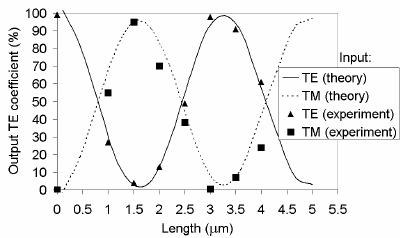
\includegraphics[width=8cm]{pics/polrot_fig3}}
    \subfigure[Output power \emph{versus} polarization angle for TE
      incoming
      light.]{\label{fig:polrot_figg:4}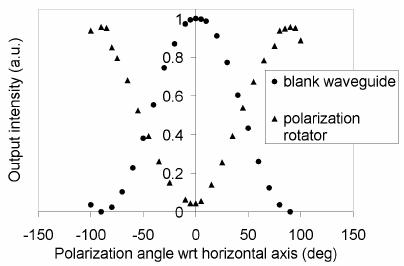
\includegraphics[width=8cm]{pics/polrot_fig4}}
  \end{center}
  \caption{Comparison between \threeDFDTD and experimental data.}
  \label{fig:polrot_figg}
\end{figure}

A good agreement between the simulation performed with a full
\threeDFDTD and the experimental results can be seen in
\figref{fig:polrot_figg:3}, assuming a slot width of $270 nm$. This
width is slightly larger than the experimentally determined width of
$230 nm$, although there is some experimental error due to the
variation of slot width with etch depth. In the following, we
therefore refer to an ``effective'' width\index{Effective!width} of $270 nm$ for the air
slots.

\figref{fig:polrot_figg:4} depicts the absolute normalized output
power as a function of the analyzer angle for a blank waveguide and a
waveguide containing a $1.5 \mu m$ long polarization rotator (the
incoming light was TE polarized for both cases). As can be seen from
the figure, the maximum output power ($100\%$) is in TE polarization
($0$ degrees) for a blank waveguide. At the same time, $96\%$ of the
output light is in TM polarization ($\sim 90\degrees$) with only $4\%$
remaining in TE polarization for the waveguide with the $1.5 \mu m$
long polarization rotator. This represents an extinction ratio of $14
dB$.

For a given width of air slots, the optimal performance of the device
strongly depends on the air/semiconductor width ratio (this ratio is
$\sim 1:1.5$ in the case depicted in
\figref{fig:polrot_figg:3}). Indeed, if the semiconductor width
increases, the grating tends to resemble a uniform slab waveguide with
tilted walls and the form birefringence is much reduced. The structure
then approximates the type of asymmetric waveguide studied previously
\cite{taillaert_compact}. Increasing the semiconductor width for fixed
air slots reduces the form birefringence due to a decreased difference
between the effective indices\index{Effective!index} of the two orthogonal eigenmodes. This
leads to a longer beat length\index{Beat length} as illustrated in
\figref{fig:polrot_optimalL_P}. For a fixed width of air slots, there
is an almost cubic dependence of the beat length on the
air/semiconductor ratio. In the other limit, for very small
semiconductor width, the form birefringence increases, but the
interface reflectivity also goes up due to increased mismatch with the
input waveguide. Device fabrication also becomes technologically more
demanding for large air/semiconductor ratios. This simulated trend is
supported by experimental evidence. A device with a $1:4$
air/semiconductor ratio and the other parameters unchanged ($270 nm$
of air slots effective width\index{Effective!width}, $1080 nm$ semiconductor width) showed an
optimal length of $30 \mu m$ \figref{fig:polrot_optimalL_P}.

\begin{figure}[htbp]
  \begin{center}
    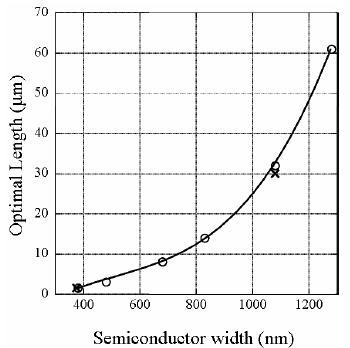
\includegraphics[width=8cm]{pics/polrot_optimalL_P}
  \end{center}
  \caption{Simulated dependence of the beat length\index{Beat length|fig} on the width of the
    semiconductor section for a $270 nm$ width of the air slots. Filled
    dots: simulated values. Solid line: cubic fit. Crosses: experimental
    values.}
  \label{fig:polrot_optimalL_P}
\end{figure}

In terms of transmitted power, we currently observe a loss of $3 dB$
(compared to a ridge waveguide without polarization rotator). The
corresponding theoretically predicted losses are around $1.5 dB$ for
deep ($\sim 2 \mu m$) slanted slots with perfectly parallel sidewalls
and $3 dB$ for similar slots with conical walls, as shown in
\figref{fig:polrot_holes}.

\begin{figure}[htbp]
  \begin{center}
    \subfigure[No holes.]{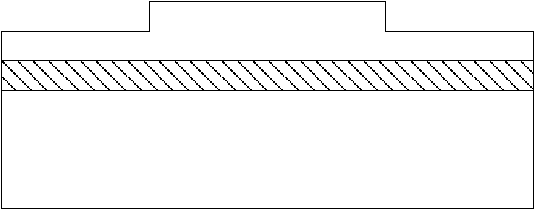
\includegraphics[width=5cm]{pics/polrot_no_holes}}
    \subfigure[Normal holes.]{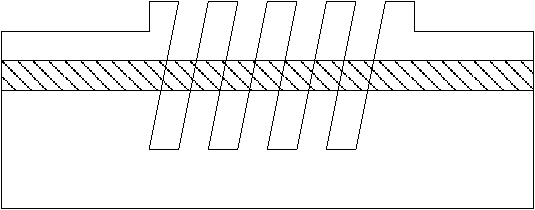
\includegraphics[width=5cm]{pics/polrot_normal_holes}}
    \subfigure[Deeper holes.]{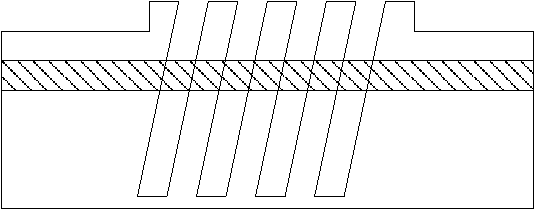
\includegraphics[width=5cm]{pics/polrot_deep_holes}}
    \subfigure[Conical holes.]{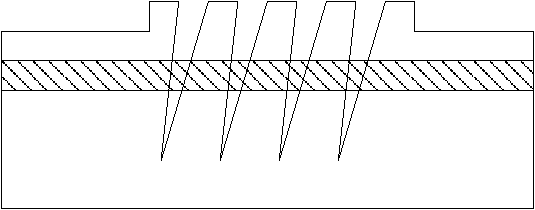
\includegraphics[width=5cm]{pics/polrot_conical_holes}}
    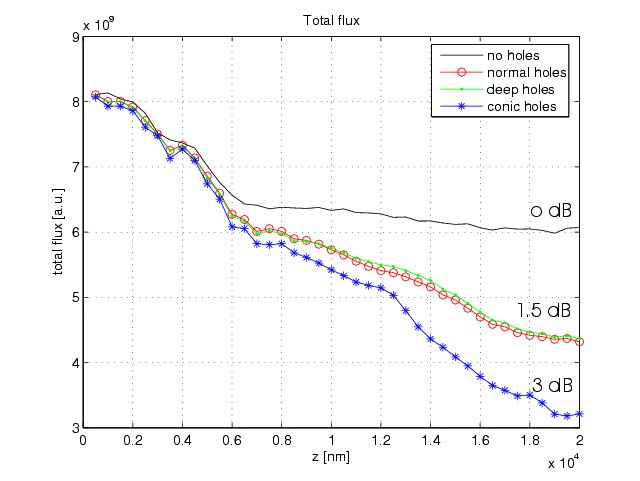
\includegraphics[width=10cm]{pics/polrot_different_holes}
  \end{center}
  \caption{Observed experimental losses are around $3 dB$, while the
    \threeDFDTD predicted losses are around $1.3 dB$ for deep slanted
    slots with perfectly parallel sidewalls. In the graph, losses for
    other kind of air slots are shown. It can be noted that $3 dB$
    losses are found for air slots with conical walls, like the one in
    \figref{fig:polrot_experimental_device}. Moreover, making the
    holes deeper has no effect: $1.6 \mu m$ etching is enough for
    losses. Note also that the initial part of the graph as little
    meaning: not a fundamental mode of the input ridge waveguide is
    inputted, therefore some power is radiated in the first $10 \mu
    m$.}
  \label{fig:polrot_holes}
\end{figure}

Thus the main source of the loss is considered to lie in the
imperfect, irregular or conical shape of the holes as well as
insufficiently deep etching. Both of these problems result in
undesirable out-of-plane scattering. These issues, however, can be
minimized by optimizing the etching regime and achieving deeper, more
parallel slots. As technology continuously improves, better slots
should be achievable in the near future. The remaining loss of $1.5
dB$ is due to the abrupt interface between the slotted and unslotted
sections. Further improvements in the interface design, such as more
adiabatic transitions, will reduce these losses to acceptable levels.
 
With respect to bandwidth, it is worth noting that the experiments
were performed at several different wavelengths in the $1290$ to $1330
nm$ range, with no compromise in performance; this clearly indicates
broadband operation, which is also supported by the predicted
wavelength window of $200 nm$ in \figref{fig:polrot_FDTD:spectrum}, in
which the extinction ratio is better than $15 dB$.

\begin{figure}[htbp]
  \begin{center}
    \subfigure[Polarization coefficient (defined as the ratio of the
      power in one polarization over the total power), for a TE input
      field.]{\label{fig:polrot_FDTD:pol_coeff}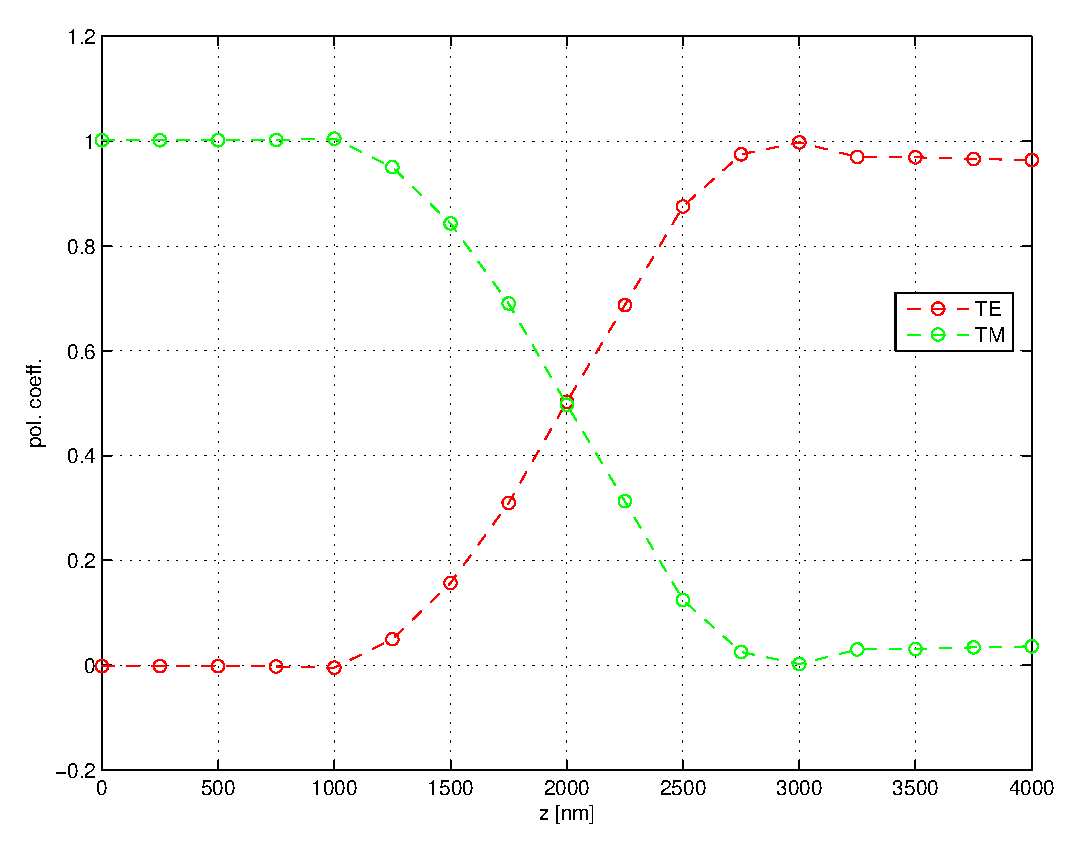
\includegraphics[width=6cm]{pics/polrot_pol_coeff}}
    \subfigure[Spectrum of the device: we achieve $15 dB$ extinction
      ratio over $200nm$ of bandwidth (yellow
      region).]{\label{fig:polrot_FDTD:spectrum}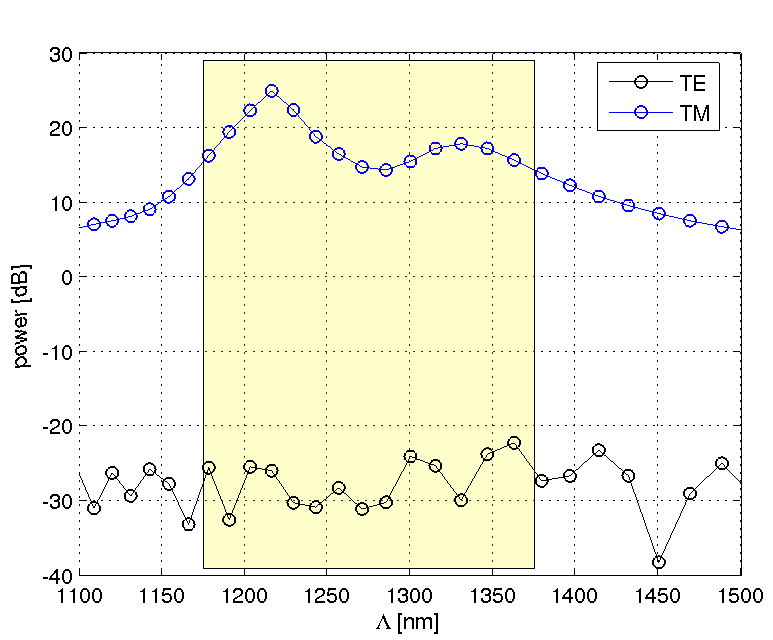
\includegraphics[width=6cm]{pics/polrot_spectrum}}
    \subfigure[Field plot (not in scale). The input TE polarization is
      transformed into the output TM
      polarization.]{\label{fig:polrot_FDTD:field}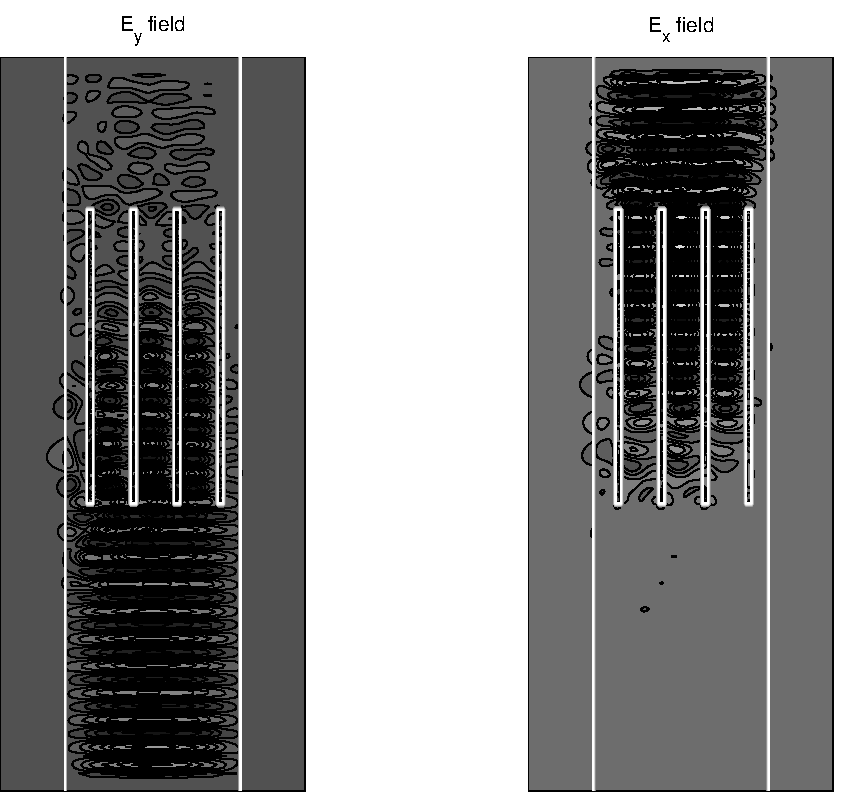
\includegraphics[width=8cm]{pics/polrot_field}}
  \end{center}
  \caption{\threeDFDTD results.}
  \label{fig:polrot_FDTD}
\end{figure}

Finally, in \figref{fig:polrot_FDTD:pol_coeff} the polarization
coefficient, defined as the ratio between the power in one
polarization over the total power, as a function of the polarization
rotator length is shown. We can note that after $1.6 \mu m$ almost all
the power has passed from TE to TM. $1.6 \mu m$, as predicted by the
\threeDFDTD, slightly differs from the $1.5 \mu m$ predicted by the mode
solver, but greatly agrees with experimental results.

\index{Polarization!rotator|)}